\section{Discrete Wavelet Transform}

%=================================================
\subsection{Background}
A wavelet is a wave-like oscillation with an amplitude that begins at zero, increases, and then decreases back to zero. It can typically be visualized as a "brief oscillation" like one recorded by a seismograph or heart monitor \cite{lipson2010optical}. As a mathematical tool, wavelets can be used to extract information from many different kinds of data, including – but certainly not limited to – audio signals and images \cite{lovis2014ehealth}.

In numerical analysis and functional analysis, a \gls{dwt} is any wavelet transform for which the wavelets are discretely sampled. As with other wavelet transforms, a key advantage it has over \gls{ft} is temporal resolution: it captures both frequency and location information (location in time) \cite{yan2014machinery}.

%Wavelet transforms have become increasingly important in digital signal processing and image processing since wavelets allow both time and frequency analysis simultaneously. The use of wavelets for these purposes is a recent development, although the theory is not new. The principles are similar to those of Fourier analysis, which was first developed in the early part of the 19th century.

In signal processing, wavelets make it possible to recover weak signals from noise . This has proven useful especially in the processing of X-ray and magnetic-resonance images in medical applications. Images processed in this way can be "cleaned up" without blurring or muddling the details \cite{leewavelet}.


%=================================================
\subsection{Discrete Wavelet Transform}
In 2-Dimensional dyadic multiresolution, a wavelet orthonormal basis in $L^2(\mathbb{R}^2)$ is built up from (tensor) products involving:

\begin{itemize}[noitemsep,nolistsep]
	\item A scale function $\varphi$ associated to a multiresolution $\{V_j\}_j\in Z$ of $L^2(\mathbb{R})$
	\item An orthonormal wavelet $\psi \,\in\, L^2(\mathbb{R})$  to define a complete
	orthonormal system, for the	Hilbert space
	\(\scriptstyle L^2\left(\mathbb{R}\right)\) of
	square integrable functions.
\end{itemize}

The orthonormal wavelet $\psi$ is constructed as the family of functions:
\begin{equation}
	\psi^k_{jn}(x) = 2^\frac{j}{2} \psi^k\left(2^jx_1 - n_1,2^jx_2 - n_2\right)\
\end{equation}
for integers \(\scriptstyle j,\, k \,\in\, \mathbb{Z}\).

For this purpose, one defines three wavelets:
\begin{subequations}
	\begin{align}
		\psi^1(x_1, x_2) &= \varphi(x_1)\psi(x_2)\\
		\psi^2(x_1, x_2) &= \psi(x_1)\varphi(x_2)\\
		\psi^3(x_1, x_2) &= \varphi(x_1)\varphi(x_2)
	\end{align}
\end{subequations}
	
\iffalse
The integral wavelet transform is the integral transform defined as:
\begin{equation}
	\left[W_\psi f\right](a, b) = \frac{1}{\sqrt{|a|}} \int_{-\infty}^\infty \overline{\psi\left(\frac{x-b}{a}\right)}f(x)dx\
\end{equation}

The wavelet coefficients \(\scriptstyle c_{jk}\) are then given by:
\begin{equation}
	c_{jk} = \left[W_\psi f\right]\left(2^{-j}, k2^{-j}\right)
\end{equation}

Here, \(\scriptstyle a \;=\; 2^{-j}\) is called the binary dilation or dyadic dilation, and
\(\scriptstyle b \;=\; k2^{-j}\) is the binary or dyadic position.
\fi


In the case of the discrete wavelet transform, the mother wavelet is shifted and scaled by powers of two:
\begin{equation}
	\psi_{j,k}(t)= \frac{1}{\sqrt{2^j}} \psi \left( \frac{t - k 2^j}{2^j} \right)	
\end{equation}
where $j$ is the scale parameter and $k$ is the shift parameter, both which are integers.

Recall that the wavelet coefficient \(\gamma\) of a signal \(x(t)\) is
the projection of \(x(t)\) onto a wavelet, and let \(x(t)\) be a signal
of length \(2^N\). In the case of a child wavelet in the discrete family above:
\begin{equation}
	\gamma_{jk} = \int_{-\infty}^{\infty} x(t)  \frac{1}{\sqrt{2^j}} \psi \left( \frac{t - k 2^j}{2^j} \right) dt
\end{equation}


This decomposition, which can be seen in Figure \ref{fig:wavelets_decomposition} \cite{cui2015application}, is repeated to further increase the frequency resolution and the approximation coefficients decomposed with high and low pass filters and then down-sampled. This is represented as a binary tree with nodes representing a sub-space with a different time-frequency localisation. The tree is known as a filter bank, see Figure \ref{fig:wavelets_bank}.


\begin{figure}
	\centering
	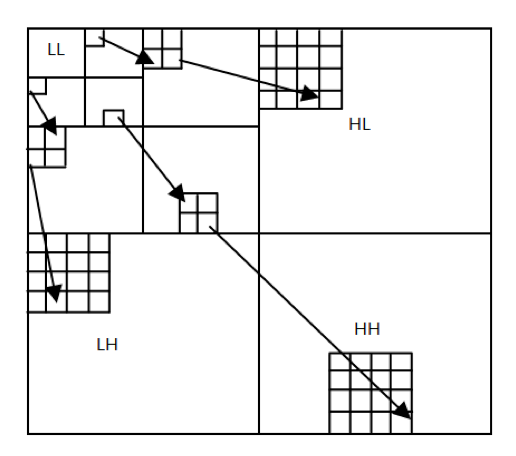
\includegraphics[width=0.4\textwidth]{fig/wavelets_decomposition}
	\caption{Wavelet coefficients arrangement}
	\label{fig:wavelets_decomposition}
\end{figure}

\begin{figure}
	\centering
	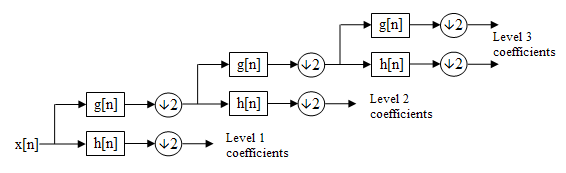
\includegraphics[width=0.8\textwidth]{fig/wavelets_bank}
	\caption{A 3 level filter bank}
	\label{fig:wavelets_bank}
\end{figure}